%%%%%%%%%%%%%%%%%%%%%%%%%%%%%%%%%%%%%%%%%%%%%%%%%%%%%%%%%%%%%%%%%%% 
%                                                                 %
%                           INLEIDING                             %
%                                                                 %
%%%%%%%%%%%%%%%%%%%%%%%%%%%%%%%%%%%%%%%%%%%%%%%%%%%%%%%%%%%%%%%%%%% 


\chapter{Werking van het programma}

In hoofdstuk drie wordt een algemeen overzicht gegeven van de opbouw en werking van het programma. Er wordt echter niet dieper ingegaan op de onderliggende code van het programma. Dit hoofdstuk zal zich voornamelijk verdiepen in deze code, de structuur ervan en zullen de belangrijkste onderdelen ervan worden uitgelegd. Hiernaast zal er ook worden beschreven hoe de externe programma's moeten worden geïnstalleerd en hoe deze in het programma worden geïmplementeerd. 
\par
Om de gedachtegang achter het ontwerpproces makkelijker volgbaar te maken zal er in dit hoofdstuk vooral gebruikt gemaakt worden van een actieve schrijfwijze en de wetenschappelijke 'we'-vorm. De code zal worden uitgelegd aan de hand van listings die rechtstreeks uit de code van het programma komen. De volledige code kan worden teruggevonden in de bijlages van deze tekst.[Bijlage D] Het is mogelijk dat de lijnnummers die in de tekst voorkomen niet volledig overeenstemmen met de lijnnummers van het gehele bestand. Dit is te wijten aan het feit dat de code kan zijn aangepast na het afdrukken van deze tekst.
\par


\section{Installatie van externe programma's}
Zoals in hoodstuk drie wordt beschreven gaan we gebruik maken van twee externe programma's die we zullen nodig zullen hebben om het programma uit te kunnen voeren, OpenBabel en PyCIFRW. Deze sectie legt uit hoe we deze kunnen installeren op een systeem. Hoewel deze in het geval van dit onderzoek met Windows 10 wordt gewerkt, werken deze software ook op oudere versies van Windows. Ons programma is gericht op besturingssysteemonafhankelijkheid, dit wil zeggen dat het ook op Linux en Apple moet werken. Het is echter mogelijk dat het installeren van deze externe programma's anders verloopt dan op Windows. De installatie van deze programma's zal in deze tekst echter enkel voor Windowssytemen worden uitgelegd.

\subsection{OpenBabel}  
De installatie van OpenBabel kan gevonden worden op hun webpagina: \url{http://openbabel.org/wiki/Category:Installation} en is gratis voor iedereen. Op deze pagina gaan we de OpenBabelGUI \textit{installer} downloaden, zie Figuur[4.1], let op dat de bit-versie met die van ons systeem overeenkomt. De download zou automatisch moeten starten. Ten slotte kunnen we de installatiewizard starten door het gedownloade bestand uit te voeren.
\par
Na het volgen van de installatiewizard zou de OpenBabel GUI moeten geïnstalleerd zijn op ons systeem, en kan het gebruikt worden in ons programma. Dit zal in het verdere verloop van dit hoofdstuk worden uitgelegd.

\subsection{PyCIFRW}
Voor de PyCIFRW module op ons systeem te installeren hebben we nood aan een prompt waarop Pyhton3.7 kan worden uitgevoerd. Zo'n prompt kan verkregen worden door anaconda te installeren en gebruik te maken van \textit{Anaconda prompt}. Vervolgens hebben we de pip installer nodig voor Python en is automatisch aanwezig op Python3.7
\par 
Pip laat ons toe allerlei Python modules te installeren, waaronder de PyCIFRW module. Dit doen we met door volgend commando in te geven in het prompt:
\begin{lstlisting}[caption=,numbers=none,language= bash]
  pip install PyCifRW
\end{lstlisting}
Dit zorgt ervoor dat we nu toegang hebben tot de PyCIFRW module wanneer we Python uitvoeren en kan eenvoudig getest worden door Python op te starten en het volgende lijn code uit te voeren:
\begin{lstlisting}[caption=,numbers=none]
  import CifFile
\end{lstlisting}

Als er geen foutmelding wordt gegeven wilt het zeggen dat de module correct is geïnstalleerd op voor onze Python installatie. 
\par
Doordat Blender een eigen Python installatie heeft zal deze nog geen toegang hebben tot onze geïnstalleerde modules. Dit kunnen we oplossen door de map die de PyCIFRW module bevat te kopiëren naar de Python installatie van Blender. Deze map kunnen we vinden op plaats waar we Python hebben geïnstalleerd op ons systeem, in het geval dat Anaconda wordt gebruikt vinden we deze in de installatiemap van Anaconda in de submap \textit{site-packages} (Anaconda3 \textgreater \textgreater{} Lib \textgreater \textgreater{} site-packages).
Vervolgens moeten we de map \textit{CifFile} kopiëren naar de Python installatie van Blender (blender-2.80.0-git.3c8c1841d72-windows64 \textgreater \textgreater{} 2.80 \textgreater \textgreater{} python \textgreater \textgreater{} lib \textgreater \textgreater{} site-packages). 
\par
Een alternatieve methode om de PyCIFRW module werkende te krijgen op Blender, zonder nood te hebben aan een Python3.7 installatie, is door de \textit{CifFile} map rechtstreeks in de Pythoninstallatiemap van Blender te plaatsen. De \textit{CifFile} kan gedownload worden vanaf de GitHub pagina van deze thesis: \url{https://github.com/JarritB/Thesis}
  
\section{Inlezen van het bestand}

\subsection{Controleren van het bestand}
Vooraleer we het bestand kunnen omzetten met OpenBabel moeten we controleren of het gekozen bestand wel dergelijk een CIF-bestand is, dit zou anders voor problemen kunnen zorgen in het verdere verloop van het programma.
\par
Om dit te controleren moeten we nazien of ons bestand de extensie \textit{.cif} heeft, in sommige gevallen wordt de extensie met hoofdletters geschreven, hiermee dienen we dus ook rekening te houden. Omdat de bestandsnaam het volledige pad naar het bestand inhoudt moeten we enkel de vier laatste tekens overhouden. Dit wordt gedaan op lijn 725 van Listing[4.1].
\par 
De variabele \textit{ext} zal nu enkel de laatste vier tekens van de filenaam bevatten. Bij een cif bestand zullen deze laatste vier altijd \textit{.cif} zijn, we moeten de variabele dus hiermee vergelijken. Door de \textit{.lower()} methode op te roepen op de extensie zal deze altijd naar kleine letters worden omgezet, en hoeven we dus geen rekening te houden met hoofdletters. In het geval dat de extensie niet gelijk is aan \textit{.cif} gaan we een foutboodschap weergeven in de terminal en gaan we in de \textit{user\_feedback} variabele ook een boodschap zetten die zal verschijnen op onze add-on, deze variabele wordt later verder uitgelegd. Omdat er een fout bestand is ingegeven zal het programma beëindigd worden met een \textit{return}, het heeft geen zin dit bestand proberen te tekenen. In listing[4.1] wordt de controle van het bestand gedaan.

\lstinputlisting[linerange={730-734},firstnumber=730,caption=Controle van de extensie]{listings/__init__.py}

\subsection{Uitvoeren van OpenBabel}
Nu we zeker weten dat we met een CIF-bestand te maken hebben kunnen we de inwendige symmetrie van het kristal wegwerken met OpenBabel. 
\par
Het oproepen van OpenBabel doen we met behulp van de \textit{subprocess} module van python. Wanneer we deze module oproepen zal er een nieuw process worden gestart, die in ons geval OpenBabel zal uitvoeren.
\par
Voor we de \textit{subprocess} module kunnen oproepen in ons script moeten we  deze importeren met de lijn code in Listing[4.2]

\lstinputlisting[linerange={13-13},firstnumber=13,caption=Importeren van de subprocess module]{listings/__init__.py}

Vooraleer we OpenBabel gaan oproepen gaan we controleren of OpenBabel wel geïnstalleerd is op ons systeem. Dit wordt gedaan met een \textit{try-except} blok, zie Listing[4.3], welke gaat proberen de code in het \textit{try} gedeelte uit te voeren. Als dit niet lukt zal het programma in plaats daarvan het \textit{except} gedeelte uitvoeren. Bij een correcte installatie van OpenBabel zal de \textit{obabel\_fill\_unit\_cell} functie worden uitgevoerd, zie lijn 739 van Listing[4.3].
\par
In het geval dat OpenBabel niet kan worden opgeroepen gaan we een foutboodschap weergeven in de terminal en in de \textit{user\_feedback} variabele en zal ons programma verder werken met het ingegeven CIF-bestand. Hoewel het kristal niet kan geconverteerd worden, zullen we toch een deel van het kristal kunnen tekenen. In sommige gevallen heeft het ingegeven kristal zelfs geen inwendige symmetrie, en heeft de gebruiker geen nood aan OpenBabel om het kristal te kunnen visualiseren.

\lstinputlisting[linerange={736-744},firstnumber=736,caption=Controle van de OpenBabel installatie]{listings/__init__.py}
\par	
De functie \textit{obabel\_fill\_unit\_cell} heeft het pad naar het ingevoerde CIF-bestan en de naam van het geconverteerde CIF-bestand als argumenten en bestaat uit slechts één lijn code. Op deze lijn roepen we de \textit{run} methode op de \textit{subprocess} module op, deze heeft als argument een \textit{string} waarin het uit te voeren commando staat zoals het in een prompt zou worden uitgevoerd. Het commando waarmee we OpenBabel uitvoeren bestaat uit volgende parameters:
\begin{itemize}
\item obabel: roept OpenBabel op
\item -icif: type van het invoerbestand, wordt gevolgd door bestandsnaam
\item -ocif: type van het uitvoerbestand
\item -O: gevolgd door naam van het uitvoerbestand
\item --fillUC: selecteert de mode waarin de symmetrie zal worden omgezet
\item keepconnect: parameter van de fillUC mode, tekent ook atomen buiten de eenheidscel
\end{itemize}
In onze code ziet het er dan als volgt uit:
\lstinputlisting[linerange={675-675},firstnumber=675,caption=Uitvoeren van OpenBabel]{listings/__init__.py}

\subsection{Zelf een parser ontwerpen}
In de vierde sectie van hoofdstuk twee werd er reeds aangehaald wat er allemaal komt kijken bij het ontwerpen van een parser. Het is me gelukt een programma[Bijlage C] te ontwerpen dat alle CIF-bestanden kan inlezen die te vinden zijn op de kristallografische databank van het IZA.\citep*{IZA1} Het parsen van deze bestanden lukte omdat deze allemaal dezelfde tekststructuur hebben. Bestanden uit databanken die werken met een andere structuur kunnen verkeerd worden geïnterpreteerd waardoor de parser nutteloos is. Het is mogelijk mijn parser aan te passen zodat, ongeacht de structuur van het CIF-bestand, een juiste interpretatie van de data kan gedaan worden. Dit zou echter veel tijd vergen en zal, gezien er reeds werkende CIF-parsers bestaan, niet worden gedaan.



\subsection{Parsen met PyCifRW}
Het geconverteerde bestand parsen gaan we doen met behulp van de CifFile module van PyCIFRW. Om toegang te krijgen tot deze module moeten we deze eerst importeren in onze code, zie Listing[4.5]. Omdat er hier een fout wordt gegeven als de module niet geïnstalleerd is, moeten we deze import omsluiten met een \textit{try-except} blok. Als de module niet kan geïmporteerd worden gaan we een variabele aanzetten zodat het programma later weet dat het een foutmelding moet geven aan de gebruiker.

\lstinputlisting[linerange={16-21},firstnumber=16,caption=Importeren van de CifFile module]{listings/__init__.py}

Met de CifFile module kunnen we vervolgens een \textit{CifFile} object aanmaken. Door de bestandsnaam mee te geven als argument zal de CifFile module automatisch het bestand parsen en de data opslaan in het object, dit wordt gedaan op lijnen 740 en 744 van Listing[4.3]. Naast het \textit{CifFile} object maken we ook een object van de \textit{Crysdata} klasse aan. Deze klasse heeft een initialisatiemethode die zal worden uitgevoerd zodra een object ervan wordt aangemaakt, zie Listing[4.6]. In deze methode gaan we de attributen van de klasse bepalen. Enkele insteressante attributen van deze klasse zijn:

\begin{itemize}
\item start: start een soort van timer op, zo kan de loopduur van het programma worden nagekeken
\item cell: een object van de \textit{Cell} klasse, bevat de roosterparameters
\item atoms: een lijst van objecten van de klasse \textit{Atom}, alle atomen van het eenheidskristal
\item pos: een lijst met alle inwendige symmetrieën van het kristal, deze wordt voorlopig niet gebruikt
\item ftoc: de fractionele naar orthogonale conversiematrix, deze wordt berekend aan de hand van de roosterparameters
\end{itemize}

In Listing[2.7] van hoofstuk twee werden de voornaamste functies van de CifFile module reeds beschreven. In hoofdstuk drie zagen we ook dat zo een \textit{CifFile} object kan gezien worden als een dictionary. Alleenstaande gegevens in het datablok van het CIF-bestand, zoals de roosterparameters, kunnen we eenvoudig opvragen met de correcte sleutels. Dit doen we om een object van de klasse \textit{Cell} aan te maken, zie Listing[4.6].

\lstinputlisting[linerange={576-583},firstnumber=576,caption=Initialisatiemethode van de klasse Cell]{listings/__init__.py}

Het toekennen van het object \textit{atoms} doen we met een aparte functie. In deze functie gaan we nieuwe \textit{Atom} objecten aanmaken, deze invullen met data door het lusblok met atom in \textit{CifFile} object te doorlopen en deze in een lijst plaatsen. Dit wordt gedaan in Listing[4.7] 

\lstinputlisting[linerange={639-659},firstnumber=639,caption=Functie die een lijst van atomen aanmaakt]{listings/__init__.py}

In de conversie die OpenBabel doet krijgen de atomen dezelfde ID toegekend als het atoom waarvan de symmetriepositie is berekend, om dit op te lossen dienen we een lijst bij te houden met de ID's van de atomen die we al hebben aangemaakt en een teller bij te houden van het aantal van atomen met deze ID. Als er een atoom met hetzelfde ID voorkomt zal er aan dit ID een nummer worden toegevoegd en gaan we de teller met één verhogen. Op deze manier zijn we zeker dat elk atoom een eigen ID heeft waarmee het later kan worden aangesproken.    

\section{Tekenen in Blender}

\subsection{Programmeren met de Blender API}
Tot nu toe zijn we in staat een CIF-bestand te converteren met OpenBabel, vervolgens te parsen met PyCIFRW en een \textit{Crysdata} object te creëren waarin de kristalinformatie staat. De volgende stap is het visualiseren van deze data in de Blender omgeving. Hiervoor gaan we gebruikmaken van de Blender API en meer specifiek, de bpy module die de Blender API aanbiedt. 
\par
Zoals met elke module die we tot nu toe gebrukt hebben, moeten we de bpy module eerst importeren. Omdat deze module niet bereikbaar is buiten de Blender omgeving gaan we weer gebruikmaken van een \textit{try-except} blok, die zal proberen de module te importeren. Als dit lukt gaan we een variabele aanzetten zodat ons programma weet dat het mogelijk is deze module te gebruiken, zoniet zal het een foutboodschap geven, maar zal alles anders wel worden gedaan zodat het programma kan getest worden buiten de Blender omgeving.
\par
Het tekenen van het kristal is een methode van de \textit{Crysdata} klasse, deze zal stap voor stap functies aanroepen waarin bepaalde onderdelen van het kristal worden getekend. Wanneer de gebruiker zich niet in de Blender omgeving bevindt zal ons programma deze methode niet oproepen. 

\subsection{Tekenen van de omkadering}

Het tekenen van de omkadering van de eenheidscel is het eerste wat er zal gebeuren. Omdat het tekenen van de omkadering een optie is de gebruker kan aanzetten, gaan we eerst controleren of deze stap wel moet gebeuren, anders wordt deze overgeslagen.
\par
De \textit{drawCell} methode is er een van de \textit{Crysdata} zelf. Deze methode zal met behulp van de conversiematrix en de roosterparameters, welke te vinden zijn in als attributen van het \textit{cell} object, eerst kleine bollen tekenen op de hoekpunten van de eenheidscel. Dit wordt gedaan in Listing[4.8]. 

\lstinputlisting[linerange={451-459},firstnumber=451,caption=Tekenen en kleuren van de hoekpunten van de eenheidscel]{listings/__init__.py}

Dit is het ideale moment om enkele, in ons programma vaak voorkomende, functies van de bpy module uit te leggen. Het aanmaken van nieuwe vormen wordt gedaan met de \textit{bpy.ops.mesh} functie. Op lijn 454 van Listing[4.8] roepen we deze functie op om een textit{primitive\_uv\_sphere} te tekenen. Deze vorm is een type van bol. In de volgende lijnen gaan we onze net aangemaakte bol als actief object zetten zodat we aan dit object een nieuw materiaal kunnen toekennen. Door een vorm een materiaal toe te kennen kunnen we een kleur geven aan het materiaal, en aan onze bol. Kleuren worden in Blender aan de hand van RBG-waarden bepaalt, deze waarden worden in de vorm van een lijst gegeven waarin het niveau van elke kleur (rood, groen, blauw) met een getal tussen nul en één wordt voorgesteld. In het geval van onze bol kiezen gebruken we de waarden [0,0,0], welke zwart voorstellen.
\par
Nu we onze hoekpunten hebben bepaald, en getekend, moeten we de ribben van onze omkadering tekenen. Dit gaan we doen door cilinders te tekenen tussen de hoekpunten van de eenheidscel. Door een lijst bij te houden waarin de bollen hoekpunten worden opgeslagen wanneer ze worden aangemaakt, zie lijn 456 van Listing[4.8], kunnen de hoekpunten worden verkregen. Omdat we niet tussen alle hoekpunten een lijn willen tekenen, dit zou namelijk ook de diagonalen tekenen, gaan we specifiëren tussen dewelke we een lijn willen tekenen. We gaan twee even lange lijsten aanmaken waarin de hoekpunten staan die we moeten verbinden. Door gebruik te maken van de \textit{zip} functie van Python kunnen we deze lijsten samennemen en er twee variabelen tegelijk over itereren. Deze twee variabelen stellen telkens een paar van objecten uit de lijst van hoekpunten voor waartussen we een cilinder gaan tekenen. Vervolgens gaan we aan de hand van de locaties van de hoekpunten de afstand ertussen berekenen, dit wordt de lengte van onze cilinder. Het tekenen van de cilinder wordt op een gelijkaardige manier gedaan als we eerder hebben gedaan bij het tekenen van de hoekpunten. De cilinder zal vertrekken op de plaats van het eerste hoekpunt en met behulp van enkele goniometrische berekeningen kunnen we de cilinder zo roteren dat het uiteinde overeenkomt met het andere hoekpunt.
\par

\lstinputlisting[linerange={464-470},firstnumber=464,caption=Samennemen van alle objecten in een vorm]{listings/__init__.py}

Ook de ribben van de cel gaan we bijhouden in een lijst. Op deze manier kunnen we na het tekenen van de ribben alle objecten uit de lijsten van hoekpunten en ribben selecteren en samenvoegen in één object. Dit wordt gedaan in Listing[4.9].     

\subsection{Tekenen van atomen}

Het tekenen van de atomen doen we met de \textit{drawAtoms} methode van de \textit{Crysdata} klasse. Deze methode zal de lijst met atomen aflopen en op elk element van deze lijst de \textit{drawObj} methode oproepen. De \textit{drawObj} methode is een methode van de \textit{Atom} klasse en wordt weergegeven in Listing[4.10] 

\lstinputlisting[linerange={609-621},firstnumber=609,caption=De tekenmethode van de klasse \textit{Atom}]{listings/__init__.py}

Om elk element een eigen grootte en kleur te geven maken we gebruik van twee dictionaries, het is mogelijk deze samen te nemen in één dictionary om minder geheugen te gebruiken, dit maakt het echter minder overzichtelijk voor de gebuiker. Door het grootte aantal elementen zijn het te veel lijnen om in het programma zelf te schrijven. Om deze reden gaan we deze dictionaries opslaan in een extern tekstbestand. Het inlezen van een dictionary vanuit een extern bestand wordt gedaan met behulp van de \textit{eval} functie. Deze functie heeft als argument een string, welke \textit{eval} als Python code zal interpreteren. Het inlezen van een externe dictionary wordt gedaan in Listing[4.11]. 
  
\lstinputlisting[linerange={88-89},firstnumber=88,caption=Inlezen van een dictionary vanuit een extern bestand]{listings/__init__.py}

De tekenmethode van het atoom zal met het symbool van het element als sleutel de straal van het atoom uit de \textit{sizedic} dictionary halen. Om de positie van het atoom te weten wordt de conversiematrix gebruikt. Deze zal de fractionele coördinaten, die atributen zijn van het atoom, omzetten naar hun orthogonale waarden. Dan tekenen we een bol met de eerder bepaalde straal op die plaats. De straal hangt ook af van de stijl waarin het kristal zal worden getekend. Bij de \textit{STICK AND BALL} stijl zal de straal worden gehalveerd, zodat de bindingen zichtbaar worden en bij de \textit{STICK} tekenstijl zal de straal zo klein zijn dat enkel de bindingen nog zichtbaar zijn. De arumenten \textit{segments} en \textit{ring\_count} op lijn 611 van Listing[4.10] bepalen uit hoeveel vlakken het de bol bestaat, bij een lage waarde zal de bol eerder hoekig zijn. Het aantal van deze segmenten kan de gebruiken kiezen en wordt aan de hand van een dictionary ingevuld.
\par
Op lijn 612 van Listing[4.10] kennen we de getekende bol een naam toe, via deze naam kunnen we onze bol later terug terugvinden in de lijst van getekende objecten. Hierna gaan we onze bol terug een materiaal en een kleur toekennen. De kleur wordt bepaald door de waarde die terug te vinden is in \textit{colordic}, dit is de dictionary waarin de kleuren van de elementen wordt gegeven. Als het kristal in de \textit{STICK} tekenstijl wordt getekend zullen de bollen steeds een witte kleur krijgen toegekend.
\par

\subsection{Tekenen van bindingen}    

In de \textit{BALL AND STICK} tekenstijl heeft de gebruiker de mogelijkheid om bindingen tussen atomen te tekenen, in de {STICK} tekenstijl zullen de bindingen steeds worden getekend terwijl deze nooit zullen getekend worden getekend in de {SPACE FILLING} tekenstijl. Het tekenen van bindingen wordt gedaan in de \textit{drawBonds} methode van de \textit{Crysdata} klasse. Deze methode zal in eerste instantie een béziercirkel tekenen en het de naam \textit{bez} toekennen, deze cirkel zal later gebruikt worden als vorm waarmee de \textit{bevel} zal worden gedaan, later hier meer over. Vervolgens gaan we de lijst van atomen doorlopen per element deze lijst nogmaals doorlopen, op deze manier kunnen we de afstand tussen elk element berekenen. Voor we deze afstand gaan berekenen gaan we eerst twee testen doen om te voorkomen dat het programma dubbel werk doet. Eerst gaan we na of de twee atomen dezelfde zijn, in dit geval zou het nutteloos zijn een binding te tekenen. De tweede test gaat in de lijst van getekende objecten kijken of er al een binding bestaat tussen deze twee atomen, zo vermijden we dat we de binding tweemaal tekenen. De \textit{bpy.data} module van de Blender API geeft ons toegang tot alle interne data van de Blender omgeving. Door \textit{bpy.data/objects} op te roepen krijgen we een dictionary waarin alle objecten kunnen worden opgeroepen aan de hand van hun ID. Doordat we onze bindingen een naam geven gebaseerd op de atomen die gebonden worden hebben we zo een manier om reeds bestaande bindingen te vinden.
\par
De gebruiker kan zelf de maximale afstand instellen die tussen twee atomen mag zijn om er een binding tussen te tekenen. De afstand tussen twee atomen gaan we berekenen met de formule:
\[ d = \sqrt{(x_{a1}-x_{a2})^2+(y_{a1}-y_{a2})^2+(z_{a1}-z_{a2})^2}\]   
Met a1 de orthogonale coördinaten van het eerste atoom en a2 die van het tweede.
\par
Enkel wanneer deze afstand kleiner is dan diegene die de gebruiker kiest moeten we een binding tekenen tussen de atomen. Hiervoor wordt de \textit{makeBond} methode opgeroepen met de twee te binden atomen als argument. Deze methode gaat eerst met de \textit{bpy.data} module de twee bollen zoeken die de atomen voorstellen. Deze twee object zullen dienen als argumenten van de volgende methode die we gaan oproepen, \textit{hookCurve}. In deze methode worden enkele, eerder abstracte, methodes van de bpy module gebruikt daarom zal deze stap voor stap worden doorlopen.

\lstinputlisting[linerange={531-532},firstnumber=531,caption=]{listings/__init__.py}

Eerst wordt er een curve aangemaakt. Deze krijgt de naam \textit{link} en het type \textit{CURVE} toegewezen. We zeggen ook meteen dat de curve driedimensionaal is, dit zorgt anders later voor problemen. Merk op dat we onze nieuwe curve niet in de lijst van objecten aanmaken, we creëren in feite een nieuwe vorm die we later als object kunnen aanmaken. 

\lstinputlisting[linerange={533-533},firstnumber=533,caption=]{listings/__init__.py}
Vervolgens gaan we nieuwe splines toevoegen aan onze curve. Splines zijn in feite lijnsegmenten waarmee een curve kan worden voorgesteld, in ons geval gaan we werken met slechts één spline die van het type \textit{bézier} is. Dit zal van onze curve een bézierkromme maken. Een bézierkromme is een manier waarop lijnen wiskundig kunnen worden voorgesteld aan de hand van twee of meer punten, die de graad van de 	bézierkromme bepalen volgens: $graad = n - 1$. Figuur[4.1] geeft een voorbeeld van een kromme die bepaald wordt door vier punten. Omdat we in ons geval enkel met rechte lijnstukken gaan werken volstaat een bézierkromme van de eerste graad en hoeven we niet dieper in te gaan op de wiskundige berekening van de vorm.

\begin{figure}[H]
\begin{center}
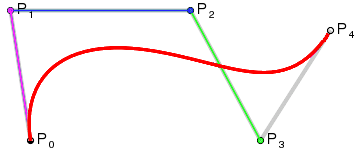
\includegraphics[]{bezier.png}
\caption{Voorbeeld van een bézierkromme met graad 3 \citep*{BEZ1}}
\end{center}
\end{figure}

Momenteel bestaat onze spline uit één bézierpunt, we moeten er dus nog één toevoegen om een lijn te bekomen.

\lstinputlisting[linerange={535-537},firstnumber=535,caption=]{listings/__init__.py}

We kennen onze bézierpunten toe aan variabelen zodat deze later makkelijk kunnen worden opgeroepen.

\lstinputlisting[linerange={544-548},firstnumber=544,caption=]{listings/__init__.py}

Nu gaan we van onze curve een object maken in de Blender omgeving. Aan zo een object kunnen we vervolgens \textit{modifiers} toevoegen aan dit object. In ons geval gaan we gebruikmaken van de \textit{hook modifier}, deze zal het object vasthechten aan een ander object. We maken een nieuwe \textit{hook modifier} aan en noemen deze \textit{alpha}. We hechten deze aan \textit{o1}, het eerste atoom, vast. Dit doen we vervolgens nogmaals voor \textit{o2}, het tweede atoom, en geven deze de naam \textit{beta}. Onze 'haken' hangen nu van aan onze atomen, maar nog niet aan onze curve.

\lstinputlisting[linerange={550-553},firstnumber=550,caption=]{listings/__init__.py}  

We gaan eerst onze curve toevoegen aan onze collectie, hierna kunnen we onze curve als actief object selecteren. Dit is nodig omdat we in de volgende lijn de tekenmode van Blender gaan veranderen naar de \textit{EDIT} mode. In deze mode worden alle hoekpunten van het actieve object zichtbaar en kan de geometrie van deze in meer detail worden aangepast. We zullen de \textit{EDIT} mode gebruiken zodat we in de volgende stap de twee bézierpunten van onze curve apart kunnen selecteren. 

\lstinputlisting[linerange={560-562},firstnumber=560,caption=]{listings/__init__.py}

Herinner dat we eerder onze twee bézierpunten aan de variabelen \textit{p0} en \textit{p1} hebben toegekend. Deze variabelen kunnen we nu gebruiken om de punten op een eenvoudige wijze te (de)selecteren. Eerst gaan we \textit{p0} selecteren en \textit{p1} deselecteren. Dan kunnen we \textit{p0} vasthangen aan de eerste \textit{hook modifier} die we \textit{alpha} hebben genoemd. Dit gaan we herhalen voor \textit{p2} en \textit{beta}. Figuur[4.2] toont een overzicht van welke \textit{modifier} welke objecten vasthecht.  

\begin{figure}[h]
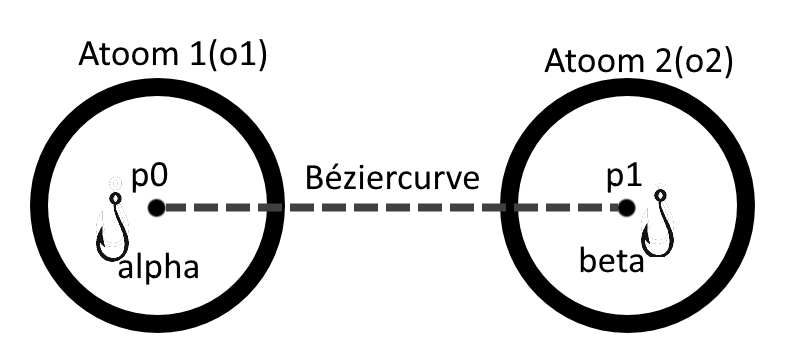
\includegraphics[scale=0.4]{hookmod.png}
\begin{tabular}{lll}
\hline
\multicolumn{1}{|l|}{Modifier} & \multicolumn{1}{l|}{Object} & \multicolumn{1}{l|}{Bézierpunt} \\ \hline
alpha                          & o1                          & p0                              \\
beta                           & o2                          & p1                             
\end{tabular}
\caption{Overzicht van de \textit{hook modifier}}
\end{figure}

Het vasthechten van objecten zal steeds gebeuren in het originepunt van een object. Als dit punt niet wordt verplaatst zal het zich steeds in het midden van een object bevinden. Hierdoor zal de curve steeds gebonden zijn aan het midden van de bollen.
\par
Hoewel we nu een curve hebben tussen onze atomen gaan we deze nog niet kunnen zien, omdat een curve geen volume heeft, zal deze niet zichtbaar zijn op het scherm. Er is nog één laatste stap die we moeten volgen om onze bindingen te tekenen, een \textit{bevel}.

\lstinputlisting[linerange={519-519},firstnumber=519,caption=]{listings/__init__.py}

In het begin van deze sectie hebben we een béziercirkel getekend, deze    



 





